\documentclass[a4paper, 11pt]{article}
\usepackage{comment} 
\usepackage{fullpage}
\usepackage{amsmath} 
\usepackage{amssymb} 
\usepackage{mathtools}
\usepackage{siunitx}
\usepackage{xfrac}
\usepackage{icomma}
\usepackage[section,below]{placeins}
\usepackage[labelfont=bf,font=small,width=0.9\textwidth]{caption}
\usepackage{subcaption}
\usepackage{graphicx}
\usepackage{grffile}
\usepackage{float}
\floatplacement{figure}{htbp}
\floatplacement{table}{htbp}
\usepackage{booktabs}
\usepackage{hyperref}

\begin{document}
\noindent
\centerline{\small{\textsc{Michigan State University}}} \\
\large{\textbf{CMSE/CSE 822 – Parallel Computing \hfill Fall 2019 \\
Homework 5}} \\
Alexander Harnisch \\
\noindent\makebox[\linewidth]{\rule{\textwidth}{0.4pt}}

\section*{1) MPI point-to-point vs collectives}
\subsection*{a)}
See code.

\FloatBarrier
\subsection*{b)}
The implementation has been timed for various numbers of sampling points (n =
1000, 100000 and 10M) and MPI processes (p = 1, 2, 5, 10, 20, 100, 250). Using
this data, the speed-up and efficiency for every data point was computed. The
results can be seen in Figure~\ref{fig:1_n_1000}, Figure~\ref{fig:1_n_100k} and
Figure~\ref{fig:1_n_10M}.

These plots have several features that can be easily understood: In all cases
(independent of the communication method used) the implementation does not
scale well with the number of used processes after a certain threshold. The
overhead produced by the parallelization is not worth it any more after that
threshold for $p$ has been reached. Where that threshold is depends on the
complexity of the problem.  For a higher complexity (larger $n$) the threshold
is also larger. This threshold can be clearly seen by a steep drop in
efficiency, which stays close to one before the threshold. 

It is also clear that The collective implementation generally clearly
outperforms the point-to-point implementation. However, that effect is a lot
stronger for larger values of $p$, which makes sense as the amount of required
communication is directly proportional to $p$. For small values of $p$ there is
almost no difference between the implementations.

\begin{figure}
  \centering
  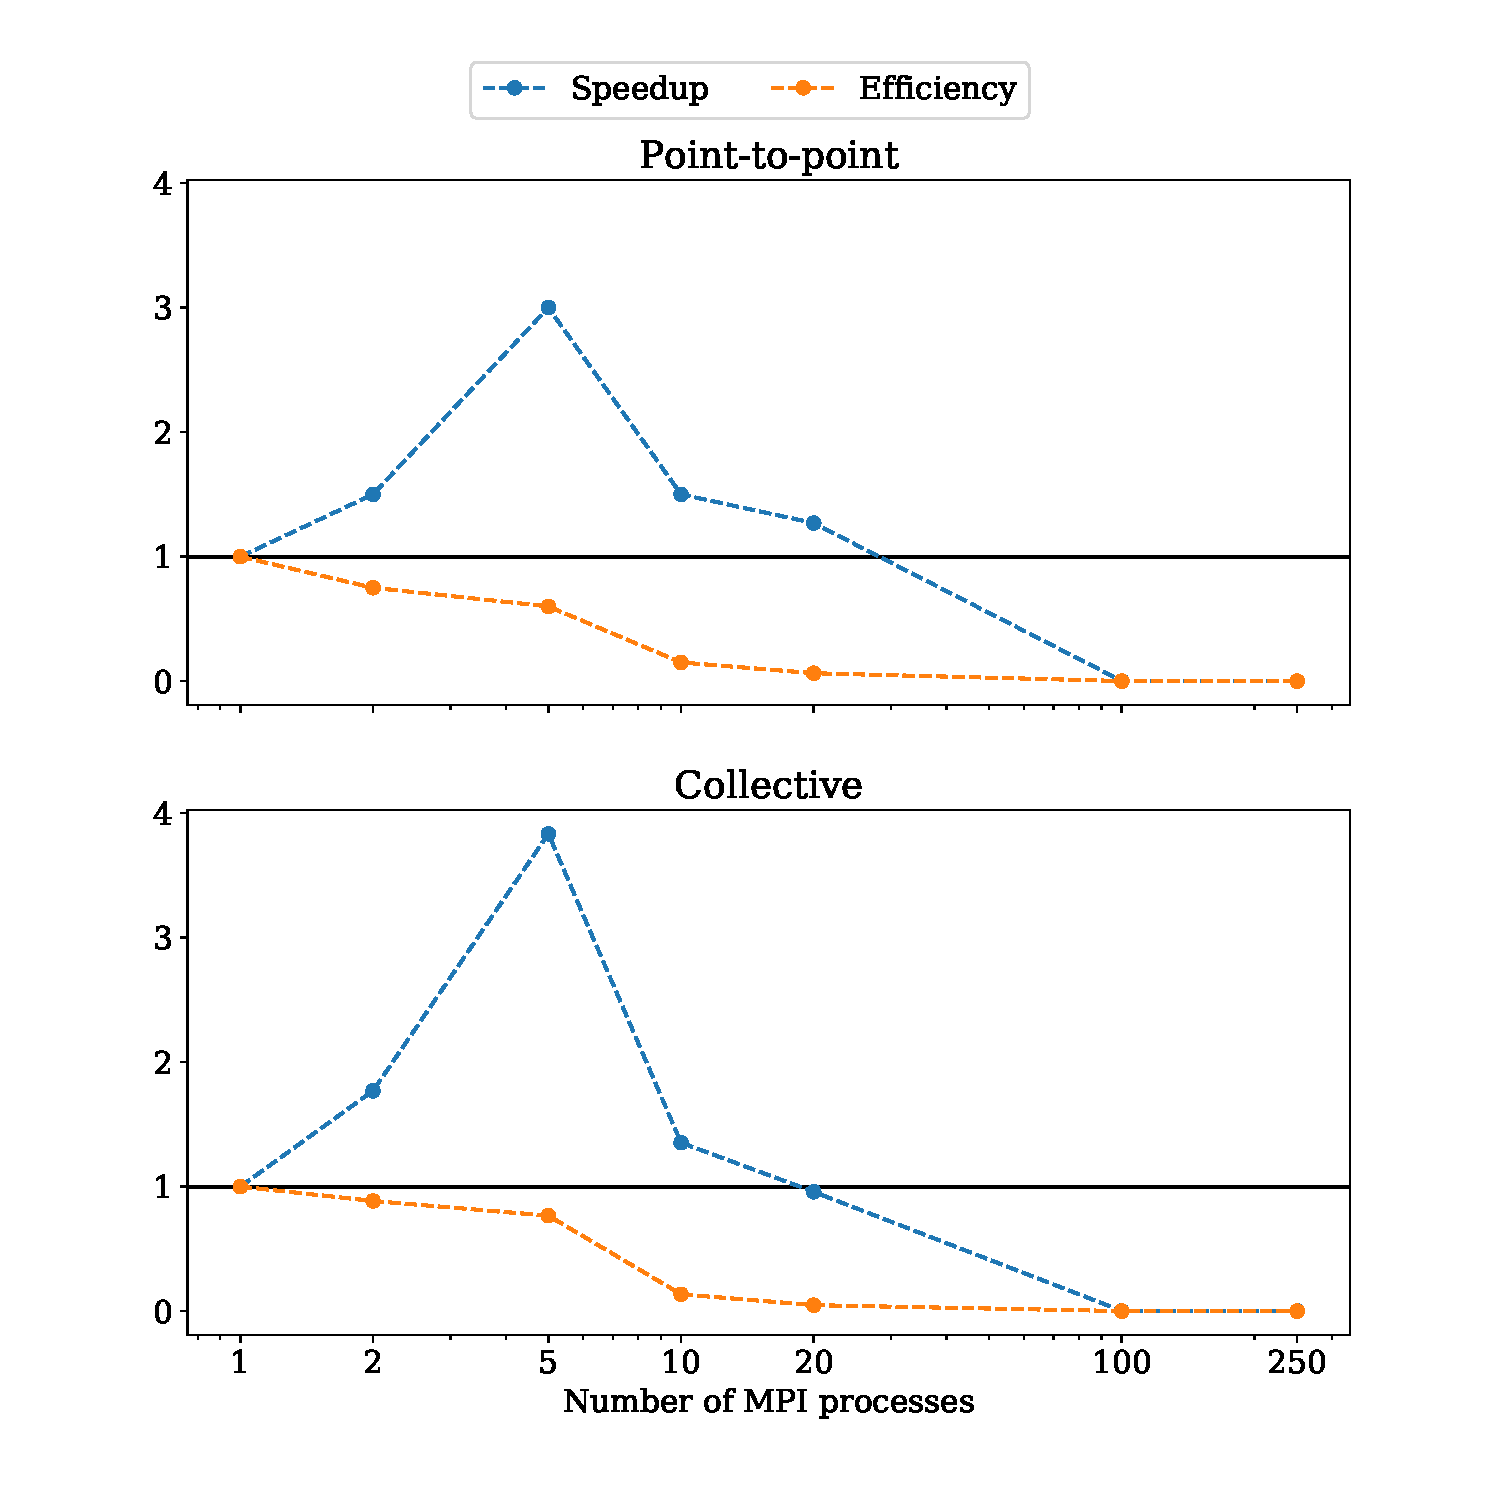
\includegraphics[width=\textwidth]{../trapezoid/plot/1000.pdf}
  \caption{Speedup and efficiency using point-to-point and collective communication for $n=1000$ sampling points.}
  \label{fig:1_n_1000}
\end{figure}
\begin{figure}
  \centering
  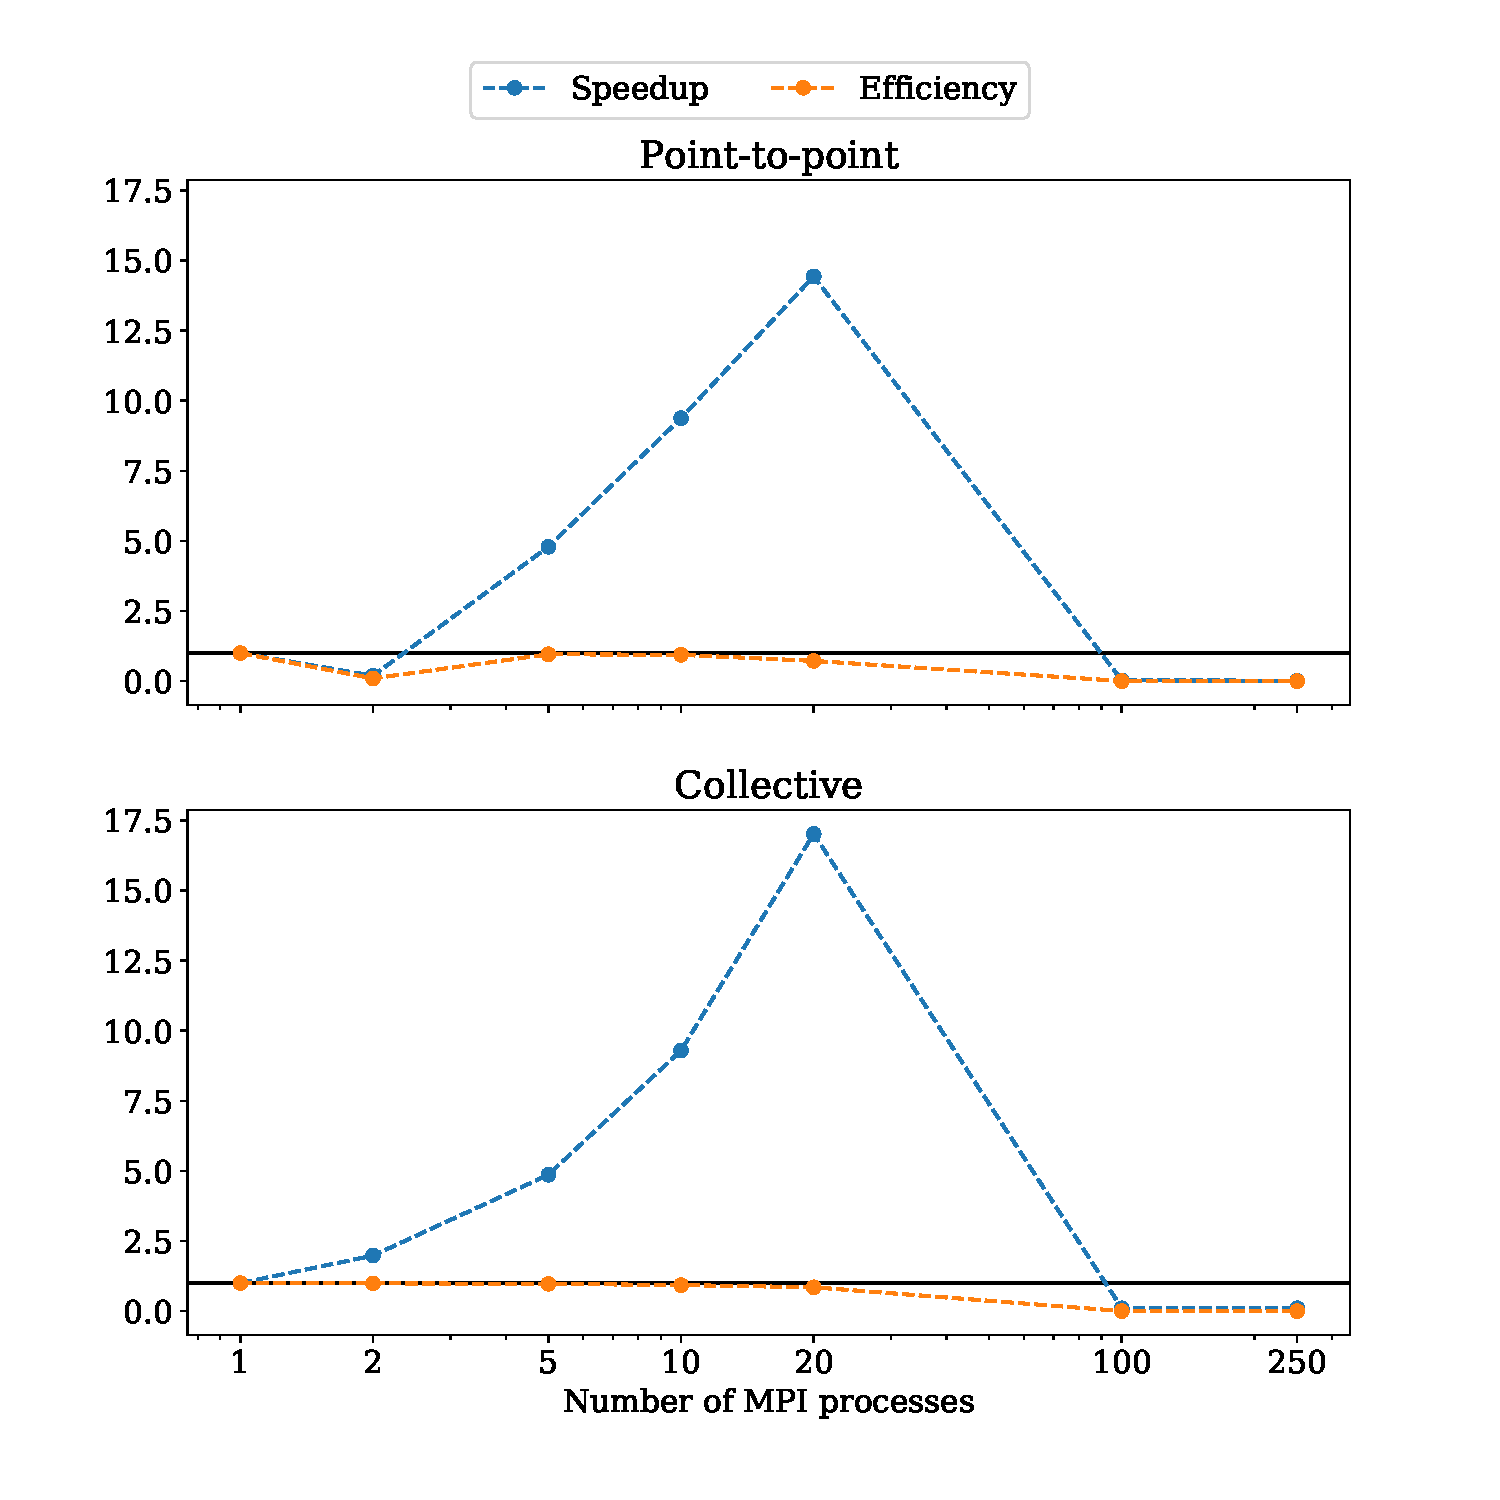
\includegraphics[width=\textwidth]{../trapezoid/plot/100000.pdf}
  \caption{Speedup and efficiency using point-to-point and collective communication for $n=10^{5}$ sampling points.}
  \label{fig:1_n_100k}
\end{figure}
\begin{figure}
  \centering
  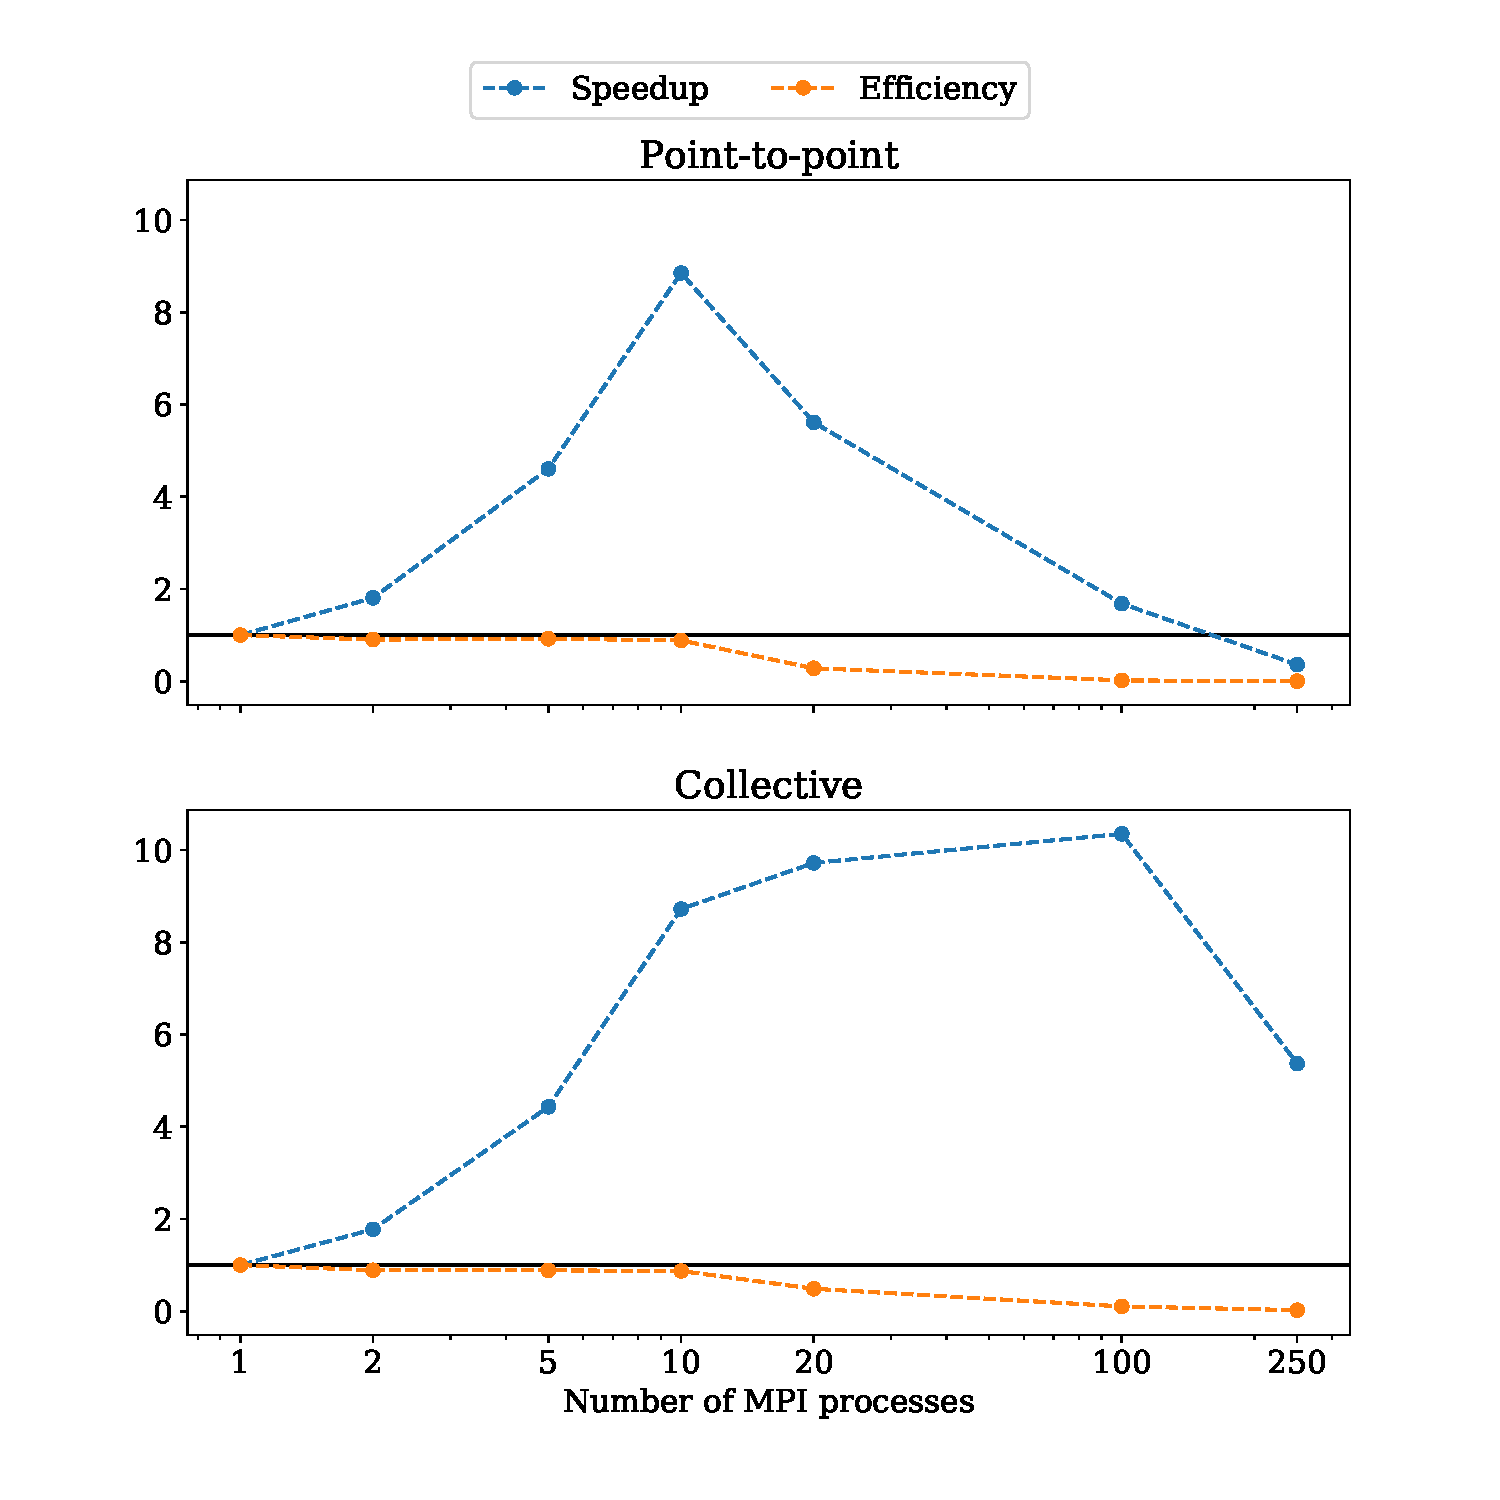
\includegraphics[width=\textwidth]{../trapezoid/plot/10000000.pdf}
  \caption{Speedup and efficiency using point-to-point and collective communication for $n=10^{7}$ sampling points.}
  \label{fig:1_n_10M}
\end{figure}

\FloatBarrier
\subsection*{c)}
The fitted parameters are listed in Table~\ref{tab:fit_paras}. The
corresponding fit results are visualized by Figure~\ref{fig:fit_1000},
Figure~\ref{fig:fit_100k} and Figure~\ref{fig:fit_10M}. The fitted model does
not take overhead into account. For that reason it is neccessary to exclude
data points that can not be described by the model. So for all fits only data
points have been used up until to the first value where the speed-up dropped
(see Figures in last subsection). In that range the model fits the data with
high accuracy, as can be seen in the figures and by looking at the small
standard deviations of the fitted parameters in Table~\ref{tab:fit_paras}.
 
\begin{figure}
  \centering
  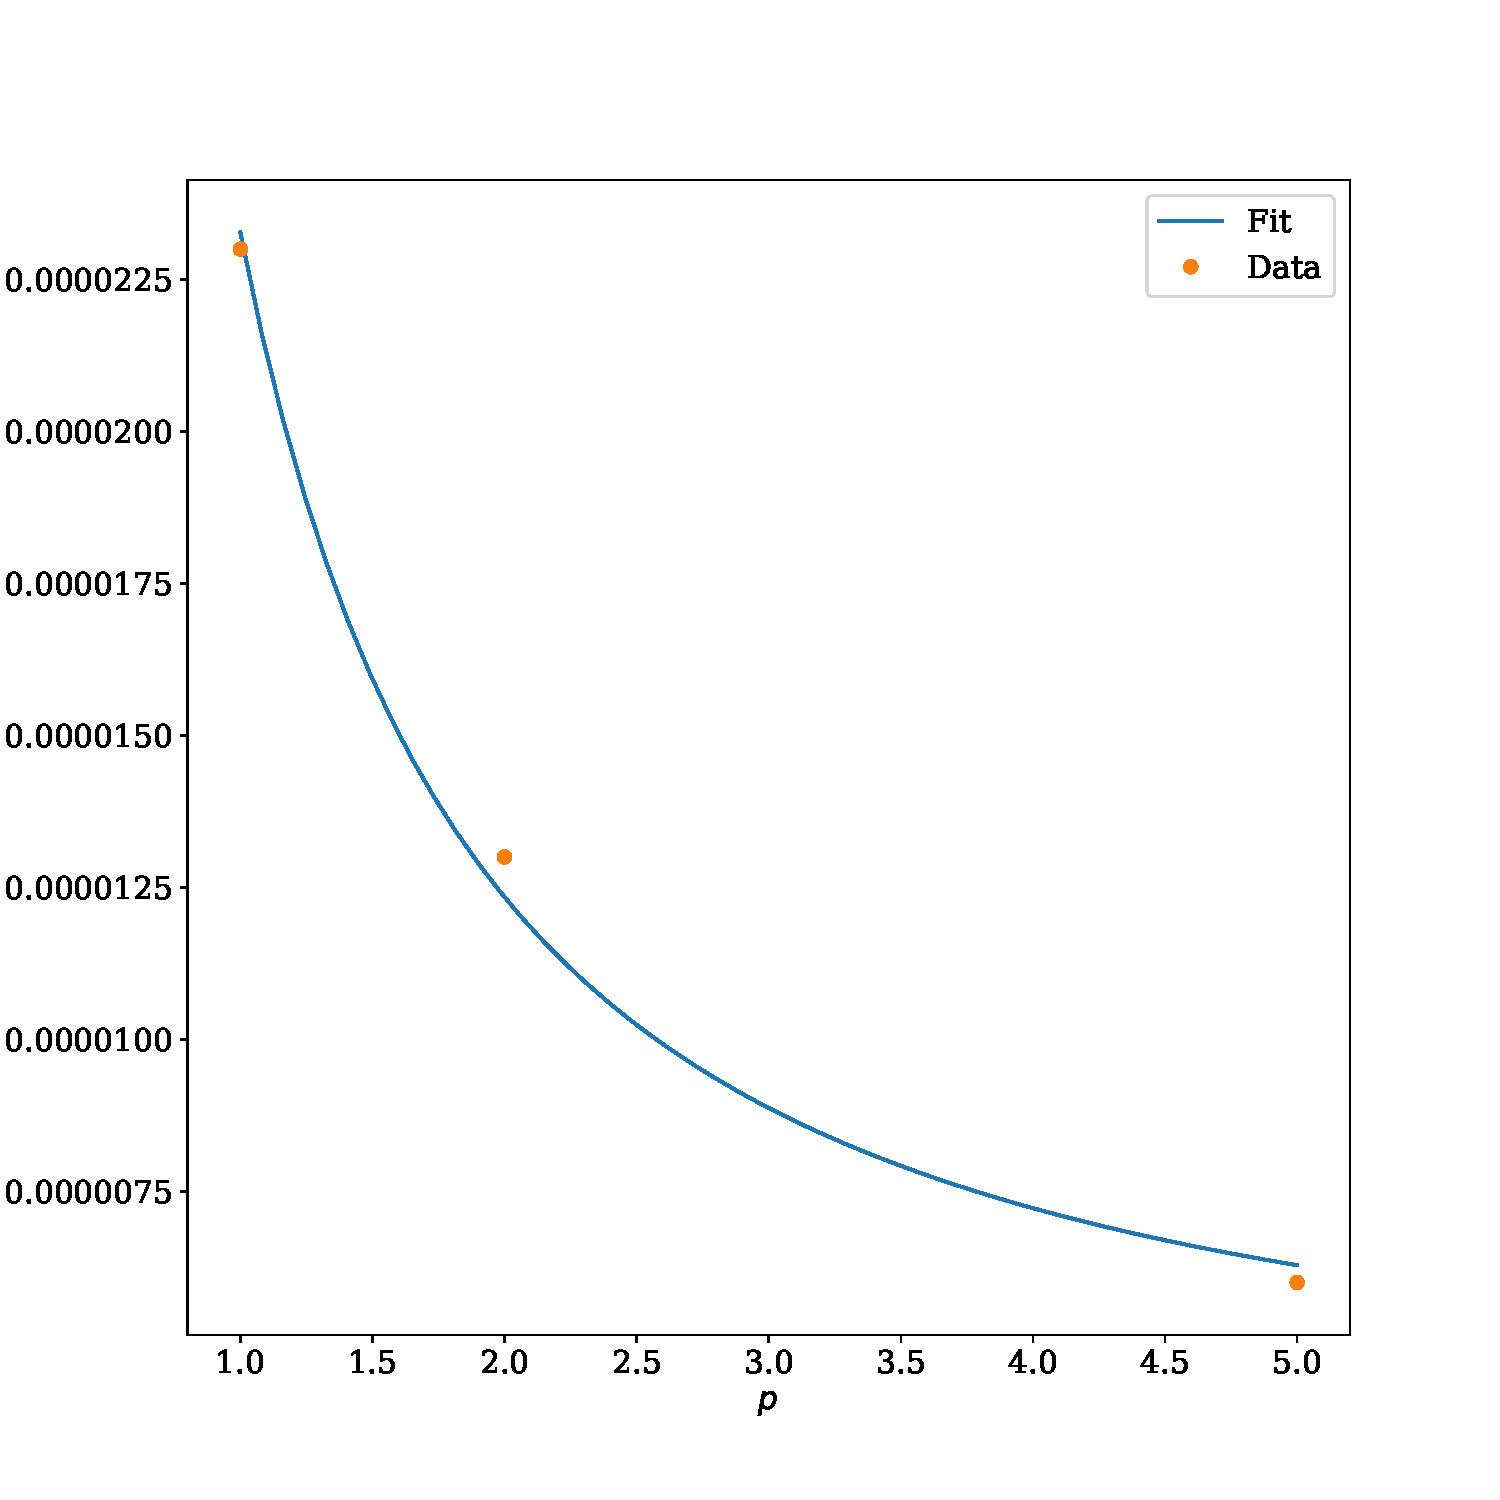
\includegraphics[width=\textwidth]{../trapezoid/plot/fit_1000.pdf}
  \caption{Least square fit for $n=1000$.}
  \label{fig:fit_1000}
\end{figure}
\begin{figure}
  \centering
  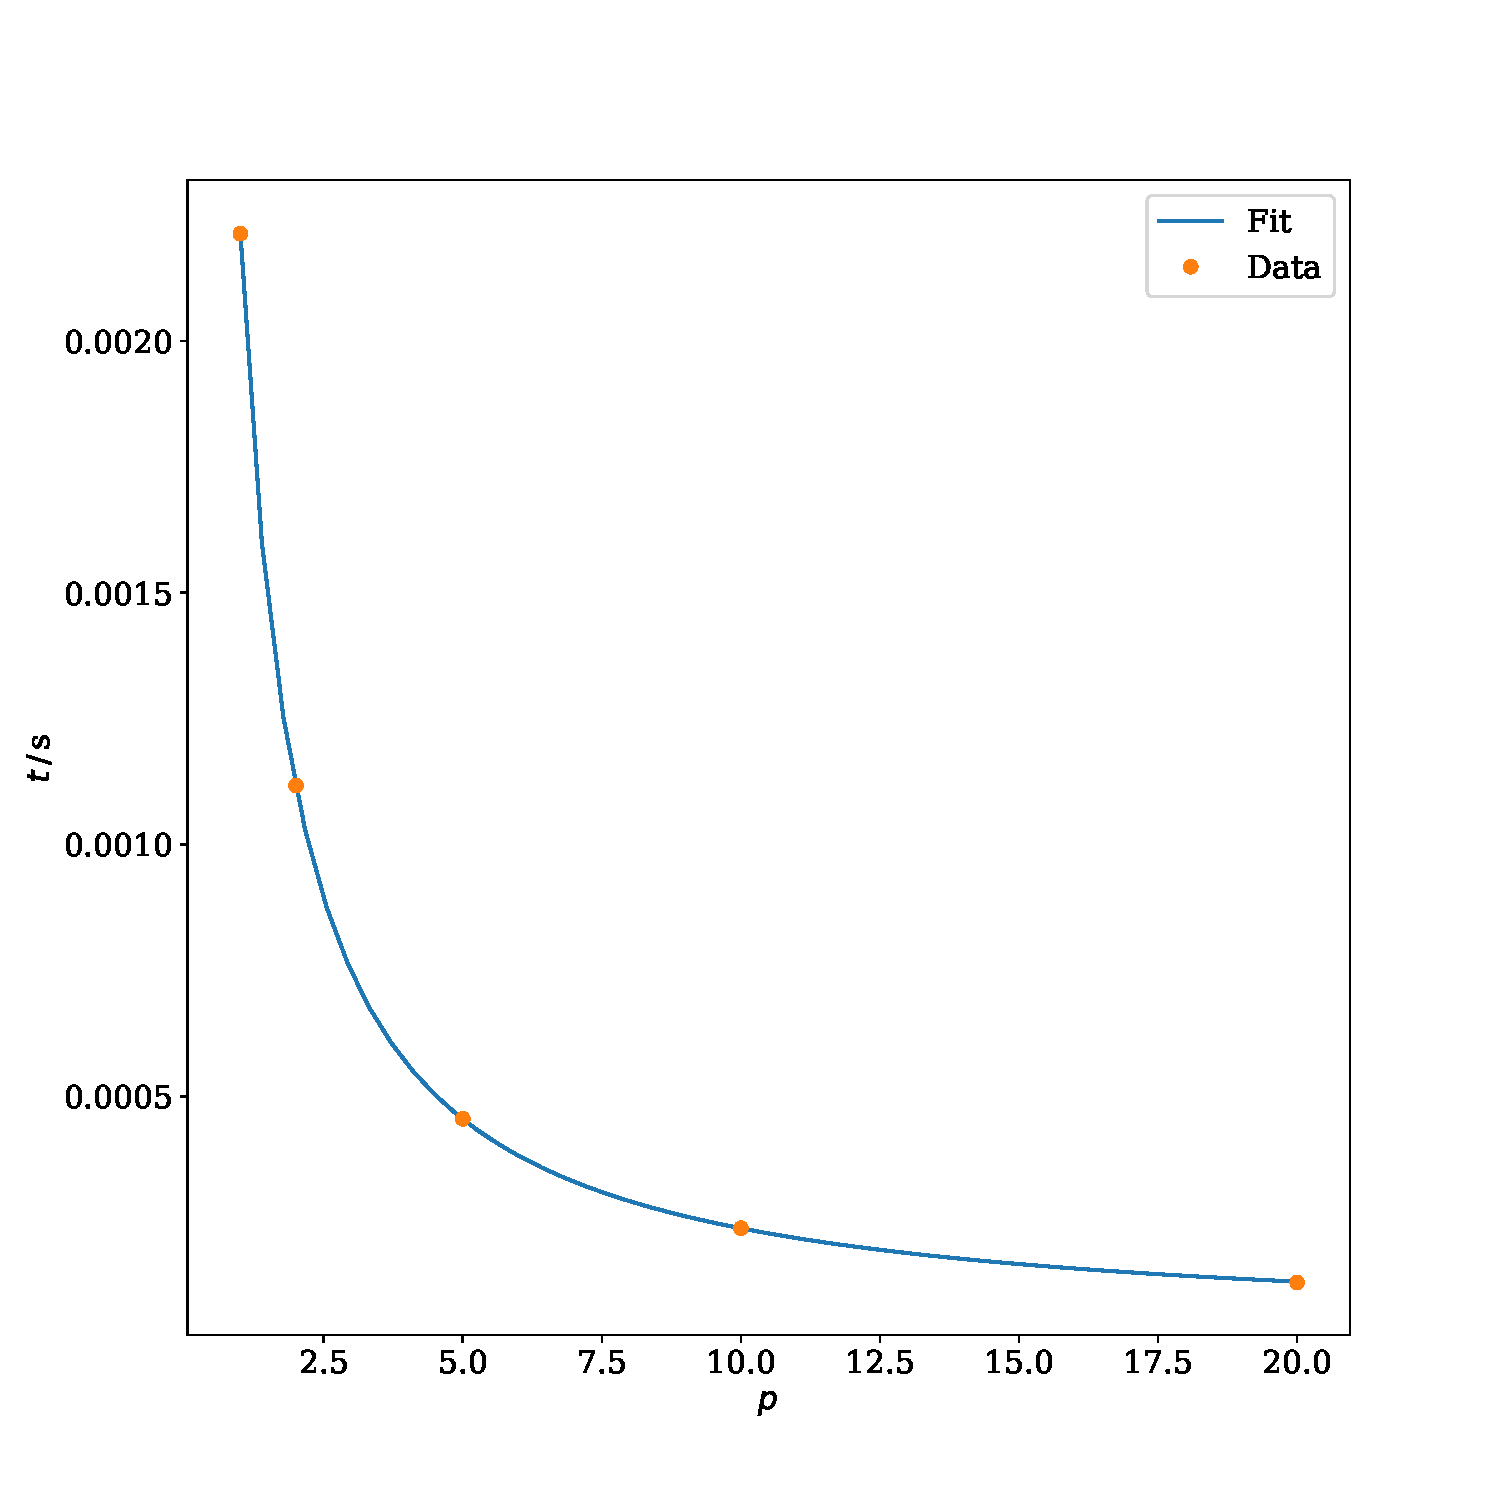
\includegraphics[width=\textwidth]{../trapezoid/plot/fit_100000.pdf}
  \caption{Least square fit for $n=10^{5}$.}
  \label{fig:fit_100k}
\end{figure}
\begin{figure}
  \centering
  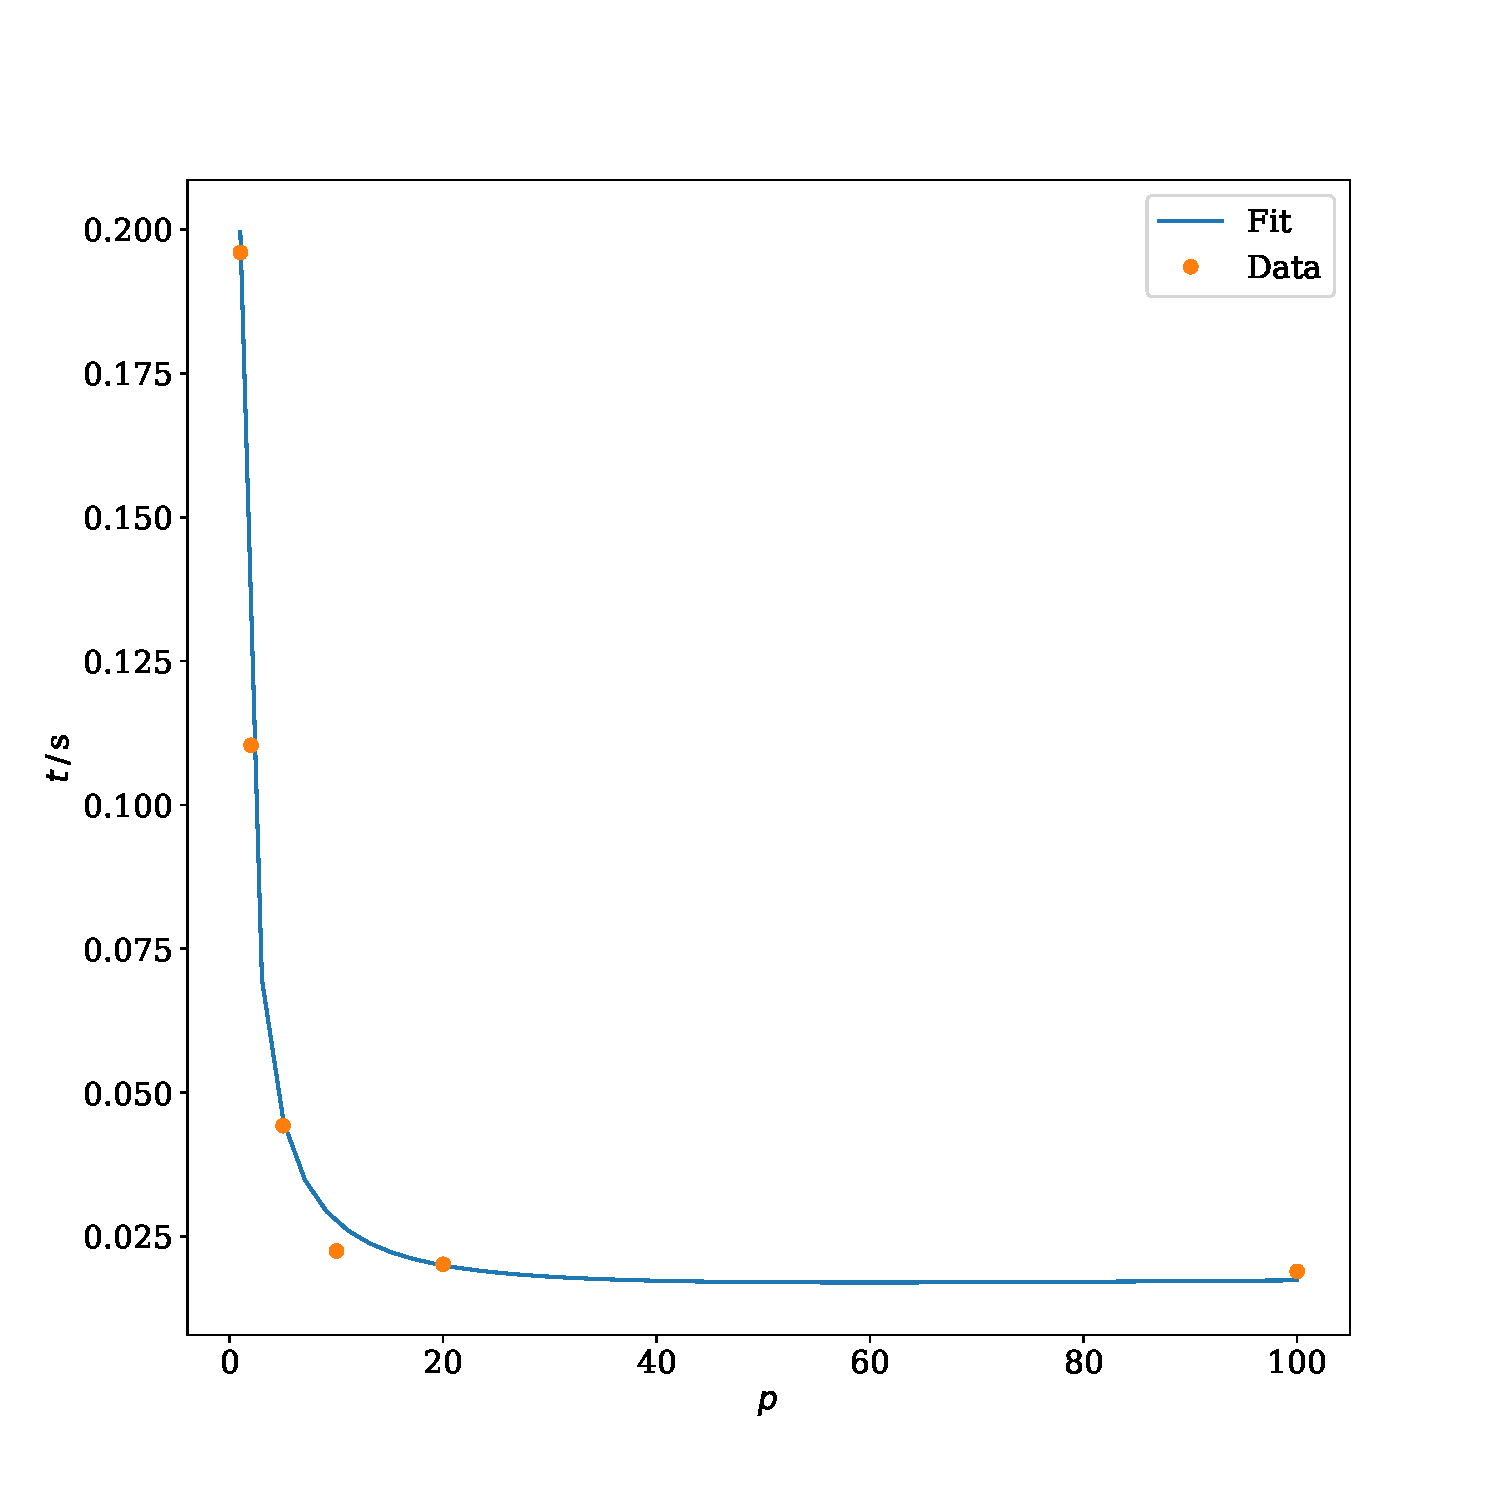
\includegraphics[width=\textwidth]{../trapezoid/plot/fit_10000000.pdf}
  \caption{Least square fit for $n=10^{7}$.}
  \label{fig:fit_10M}
\end{figure}
\begin{table}[ht]
\small
\begin{tabular}{lll}
$n$      & a / s                                          & b / s                 \\
\hline
$10^{3}$ & 2.327363481111708e-08 $\pm$ 7.198806692920759e-10 & 7.020128452971986e-07 $\pm$ 3.234141860026084e-07 \\
$10^{5}$ & 2.2153350279079064e-08 $\pm$ 2.7982074194404577e-11 & 4.843159937388218e-06 $\pm$ 5.3147319516767e-07 \\
$10^{7}$ & 1.9949962301415306e-08 $\pm$ 4.67814210500844e-10 & 0.0023154202059335717 $\pm$ 0.0005960271517657326 \\
\end{tabular}
\caption{Fitted parameters for the run time using collective communication.}
\label{tab:fit_paras}
\end{table}

\subsection*{BONUS: MPI/OpenMP parallelization}

\section*{2) Code Breaking}

\end{document}
